Figure \ref{fig:img42_src} shows  Image4\_2 which has to be restored. This image  compared to the original  (Figure \ref{fig:orignal}) has some both horizontal and vertical stripes.   Based on the frequency spectrum of this image, it can be seen that some frequency component exist around the center frequency creating this effect. The purpose of this restoration will be to reduce the effect of these component, and reconstruct it so it resembles Figure \ref{fig:orignal}

\begin{figure}[H]
    \centering
    \begin{subfigure}[b]{0.23\textwidth}
        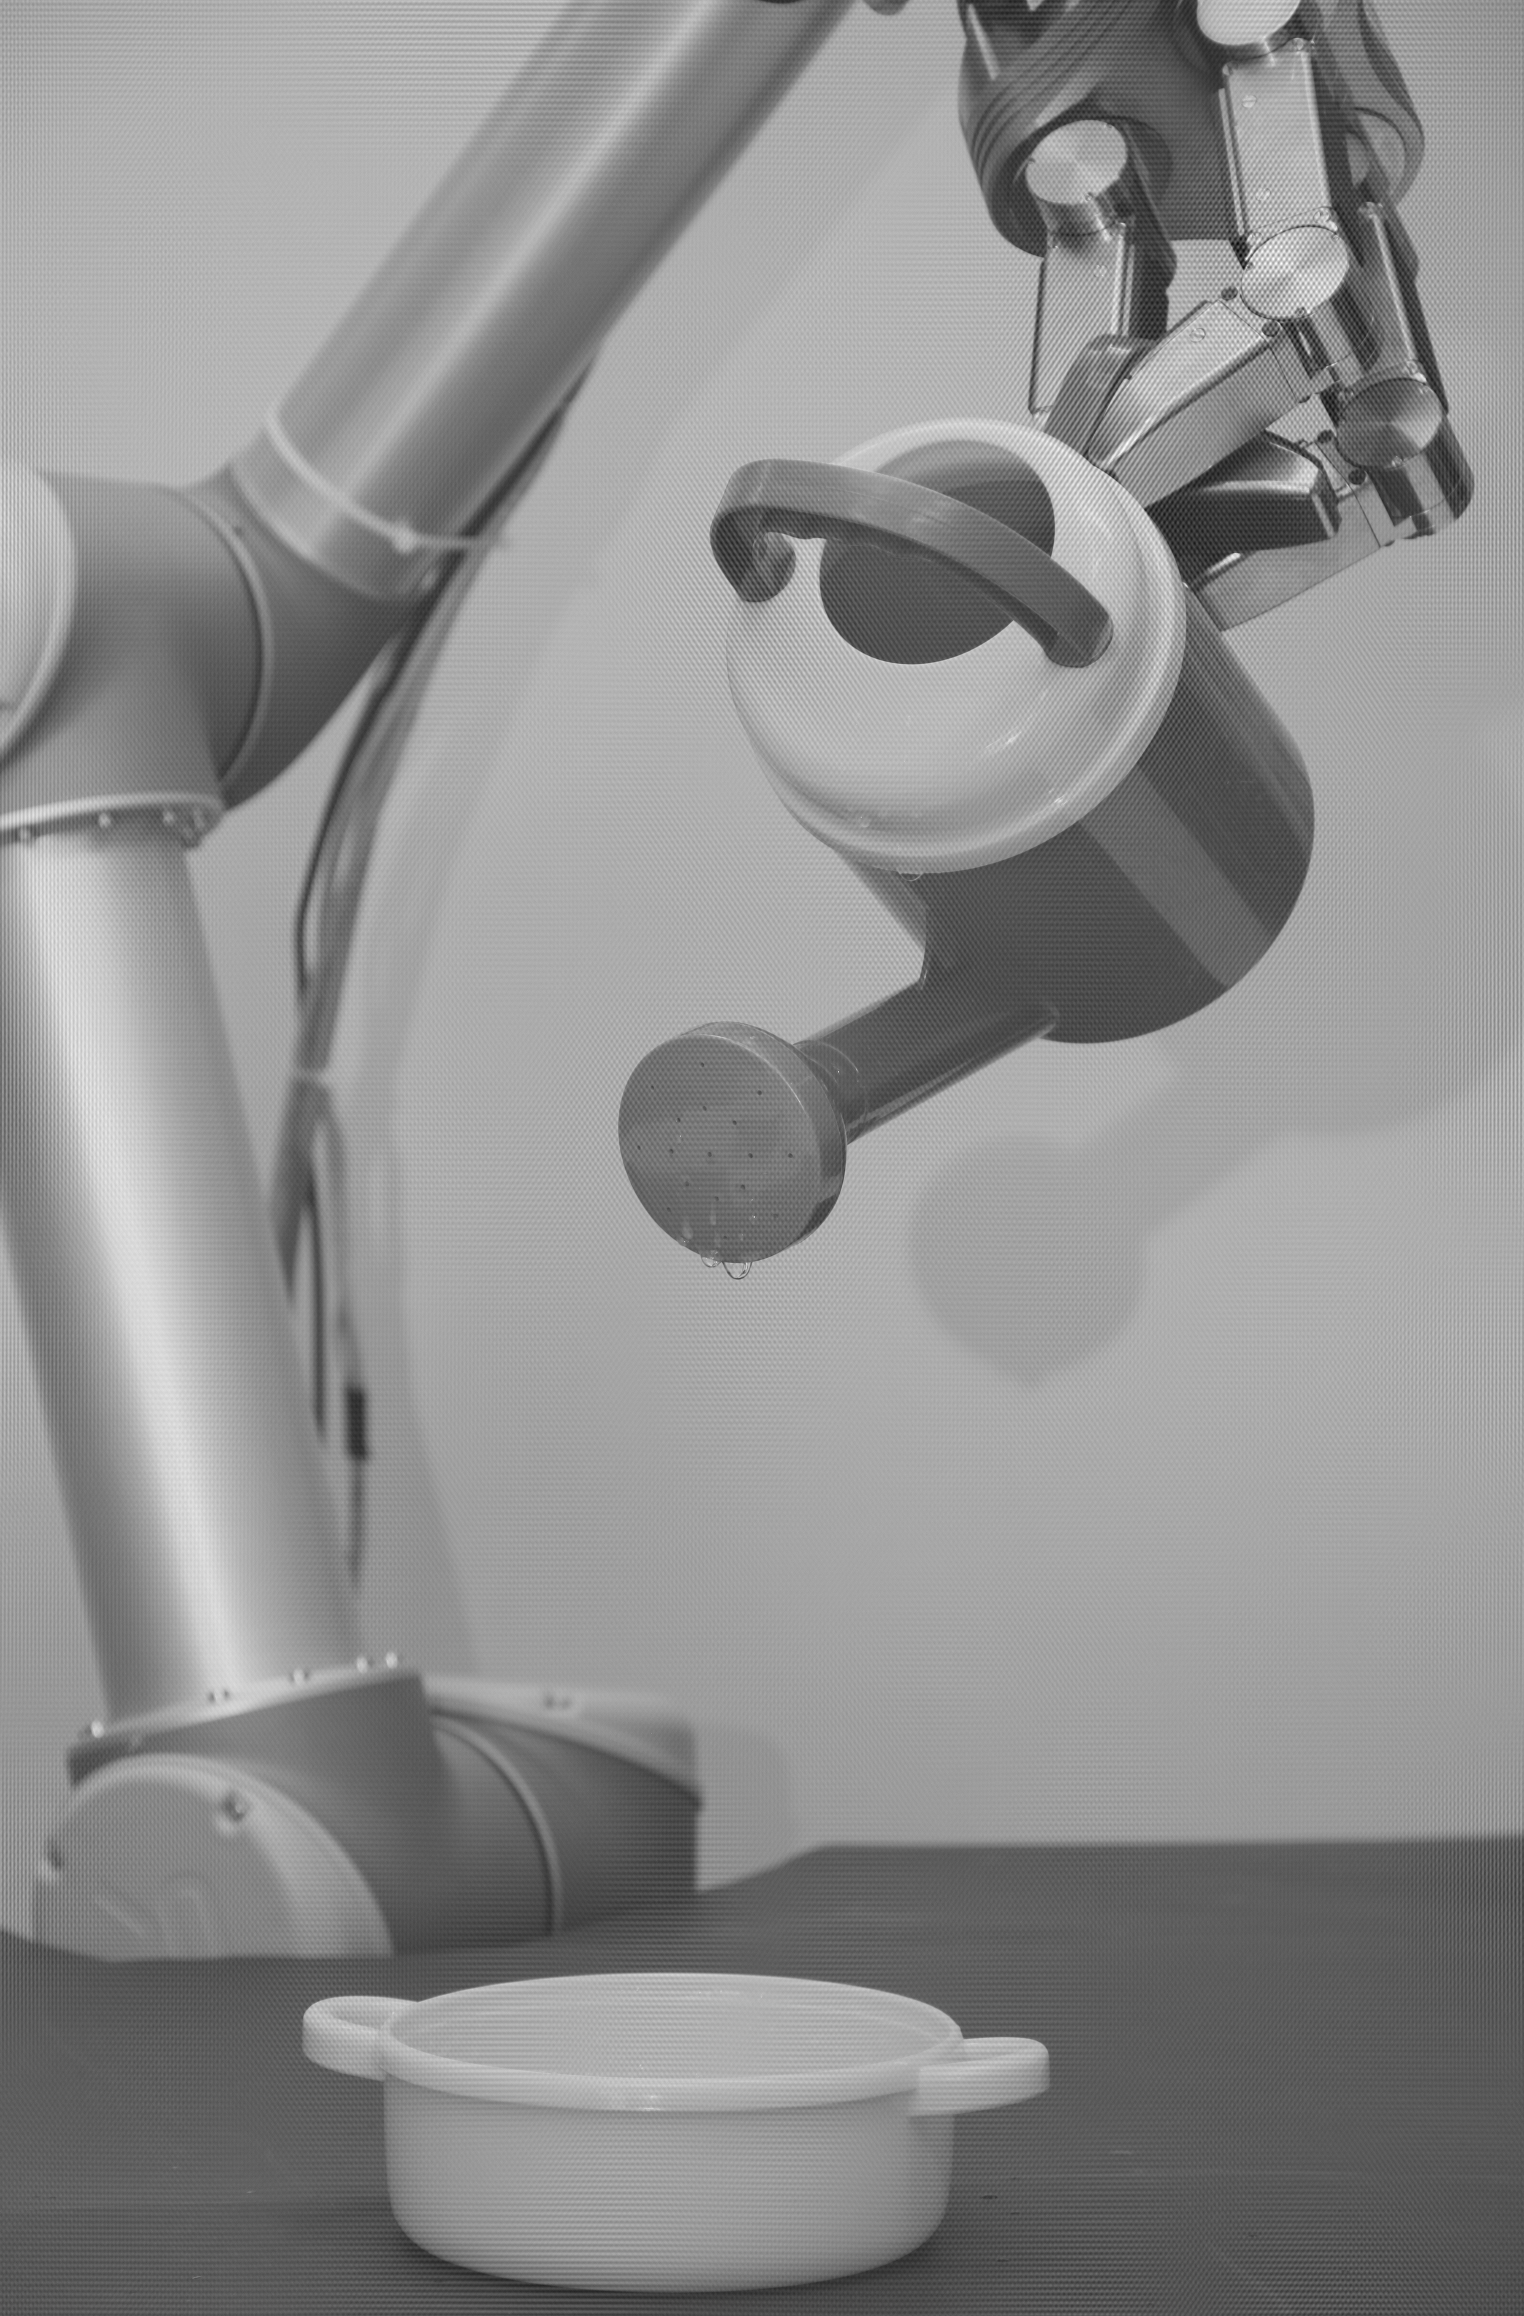
\includegraphics[width=\textwidth]{img4/Image4_2.png}
        \caption{Image4\_2 with \\no restoration}
        \label{fig:img42_src}
    \end{subfigure}
    \begin{subfigure}[b]{0.23\textwidth}
        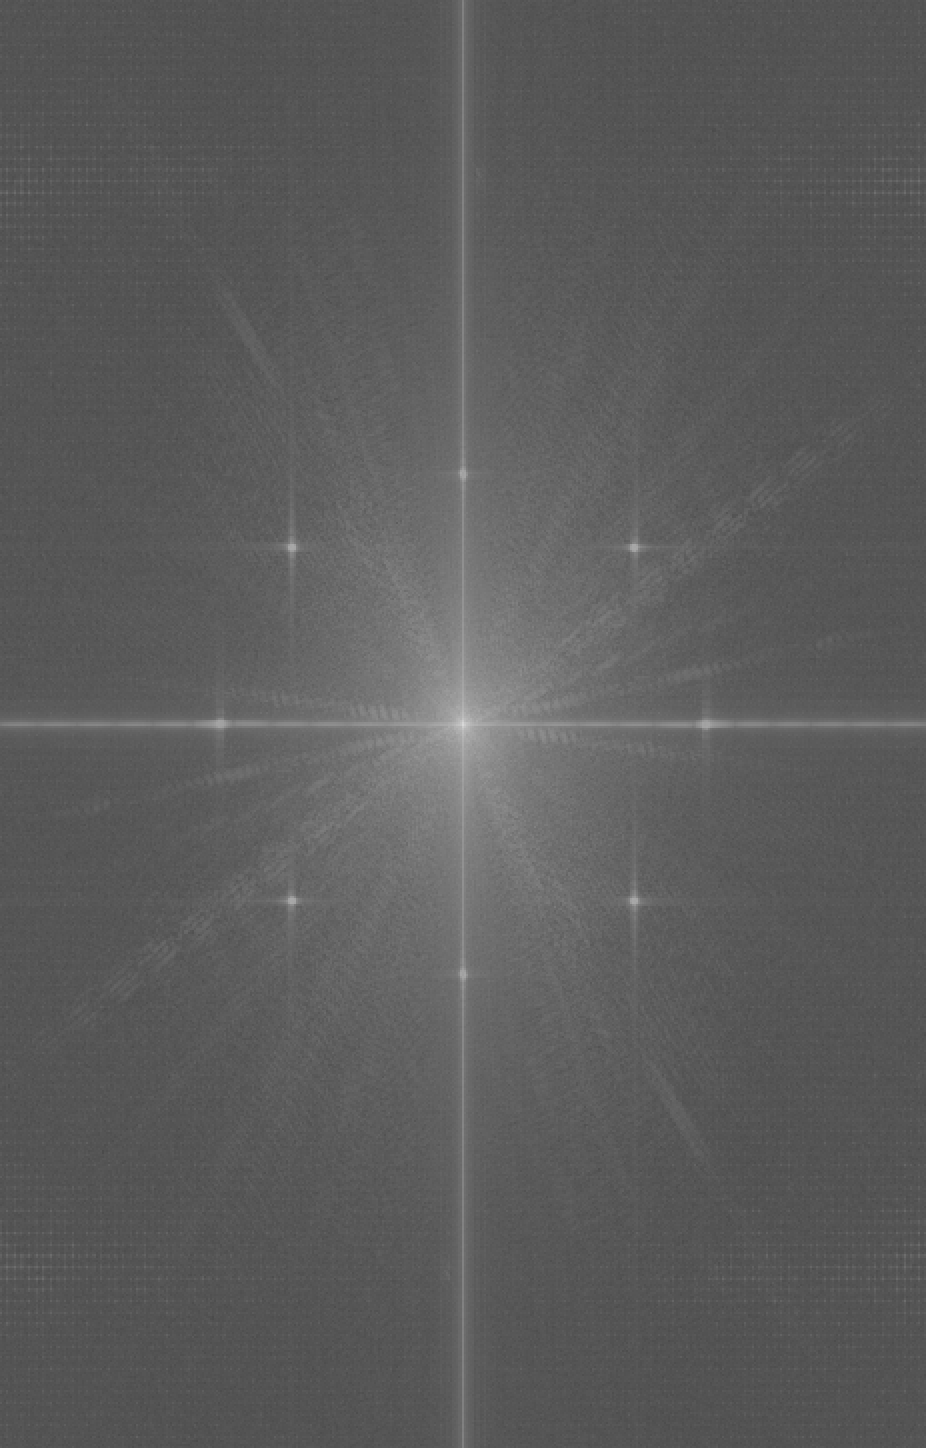
\includegraphics[width=\textwidth]{img4/Image4_2_freq_spec.png}
        \caption{Frequency spectrum of Image4\_2}
        \label{fig:img1_hist}
    \end{subfigure}
    \caption{Analysis of image 1}\label{fig:img1}
\end{figure}

The frequency components creating the circle are reason why the the stripes are occuring in the image.  One way of resolving this issue is to create a low pass filter, which let everything below a certain frequency pass, and the filter frequencies above away. \\

One type of lowpass filter is the butterworth lowpass filter which is defined as
\begin{equation}
	H(u,v) = \frac{1}{1+[\frac{D(u,v)}{D_0}]^{2n}}
	\label{eq:LBP}
	\cite{Bogen side 295}
\end{equation}
\todo{Cite til bogen side 295}
$D_0$ is the cutoff frequency given as the distance from the origin, n  is the order,  and D(u,v) is distance between a point (u,v) in the frequency domain and the center frequency rectangle, it is calculated as such. 

\begin{equation}
D(u,v) = [(u-P/2)^2 + (v-Q/2)^2]^{\frac{1}{2}} 
\end{equation}

P and Q is the padded size of the rectangle. \\


The cutoff frequency can easily by found, by computing the distance between the origin and the corresponding frequency component. 

